\documentclass[twocolumn,10pt]{article}
\usepackage[T1]{fontenc}
\usepackage[utf8]{inputenc}
%\usepackage[english]{babel}
%\usepackage{biblatex}
\usepackage[margin=1in]{geometry}
\setlength{\columnsep}{33pt}
\setcounter{secnumdepth}{2}
\usepackage{minipage-marginpar}
\newcommand\vfilbreak[1]{\vskip 0pt plus #1 \penalty-200 \vskip 0pt plus -#1}
\newenvironment{mpmp}[1]
               {\begin{minipagewithmarginpars}{#1}}
               {\end{minipagewithmarginpars}}
\usepackage{morefloats}
\usepackage{booktabs}
\usepackage{color}
\usepackage{graphicx}

\title{Lung Cancer Detection with \\Region Enhanced 
Multiple Instance Networks}
\author{Jay DeStories, Jason Fan, Alex Tong}
\date{March 2017}

\newcommand{\red}[1]{{\color{red}#1}}
\newcommand{\temp}[1]{{\red{#1}\\}}

\begin{document}

\maketitle
\section{Introduction and \\Problem~Statement}
The problem of image segmentation and structure annotation within the 
field of biomedical imaging has become a well developed and very active field in
the past years. In 2016 and 2015, the LUng Nodule Annotation (LUNA) challenge and 
SPIE Lungx challenge, asked researchers to develop models to identify pulmonary 
nodules in lung CT slices. With the 2016 LUNA Challenge, researchers gained access
to annotated CT slices that contained segmentation ground truths for abnormal 
nodules but did not release data about the malignancy of the nodules. 
In the 2015 SPIE less than 80 CT annotated images of malignant nodules were 
released to the public.

Finally, with the 2017 Kaggle Data Science Bowl, a larger dataset of
1000+ lung CT images in DICOM format was finally released with cancer/no cancer 
labels. This has allowed researchers to answer a deeper question about lung CT
scans; whether or not there are indicators of malignancy and cancer in a patient's
CT scan.

There is, however, one caveat to the Kaggle dataset. 
Although the presence of malignancy is indicated by global, binary 
cancer/no-cancer label, the location of malignant nodules and structures are
\textit{not} annotated in the training data.

Inspired by recent work in biomedical image segmentation
\cite{DBLP:journals/corr/ChristEETBBRAHD16}, region proposal 
networks and multiple instance learning for whole mammogram classification
\cite{Maron:1998:FML:302528.302753},
We seek to present a novel pipeline for lung cancer detection that enhances
multiple instance learning with region proposal.

\section{Related Work}

Over the past decade there has been a significant amount of work towards 
computer aided diagnosis of lung cancer \cite{cad_1998}. Depending on what kind
of data researchers have had access to, previous efforts to identify lung cancer
can be categorized by two main approaches. 

(1) Pulmonary Nodule Detection methods use 
image processing techniques to segment and annotate nodules
\cite{FeatureBasedLungNoduleDetection_2017, 
     LungNoduleDetectionWeaklyLabeled_2016, U-net_2015}. These methods
mimic radiologists by looking for abnormalities in the form of
``solitary white nodule-like blob[s]" in a chest x-rays and CT scans.
Lung nodules are potential cancer indicators, and as such are an important part 
in early lung cancer diagnosis. However, not all pulmonary nodules are malignant
and many are benign, there will be false positives in diagnosis if we naively
associate nodule presence with cancer. 

%\red{HELP I MADE THIS TERM UP}
(2) Direct inference and classification methods
instead attempts to directly predict the probability of cancer using x-ray and
CT images without nodule detection

\cite{Kuruvilla_2013, classificationOfNodules_2016}. 

One challenge that almost all researchers in biomedical image inference face is 
the problem with datasets being small and weakly labeled. Images labeled with
cancer/no-cancer binaries are weakly labeled because imaged tissues only display
malignancy locally; not \textit{all} of the tissue in an image will have cancer.
Multi-Instance Networks have been trained from binary labels to classify whole
mammogram images \cite{Maron:1998:FML:302528.302753}.

\subsection{\red{Reference Papers}}
\begin{itemize}
  \item Automatic Liver and Lesion Segmentation in {CT} using Cascaded Fully
    Convolutional Neural Networks and 3D Conditional Random Fields
    \cite{DBLP:journals/corr/ChristEETBBRAHD16},
  \item Deep Multi-Instance Networks with Sparse Label Assignemnt for Whole 
    Mammogram Classification \cite{Maron:1998:FML:302528.302753},
  \item U-Net: Convolutional Network for Biomedical Segmentation
    \cite{U-net_2015}.

\end{itemize}

\section{Method/Algorithm/Pipeline}
% \temp{PIPELINE: NODULE EXTRACTION -> CNN -> CANCER CLASSIFICATION}
% \temp{Will we even use RNN? If so is UNET an RNN?}
% \temp{What kind of augmentations can we do in 3d? in the z axis?}


\subsection{\red{Architecture Overview}}
Our Lung Cancer detection method uses nodule annotation to enhance direct
classification. 
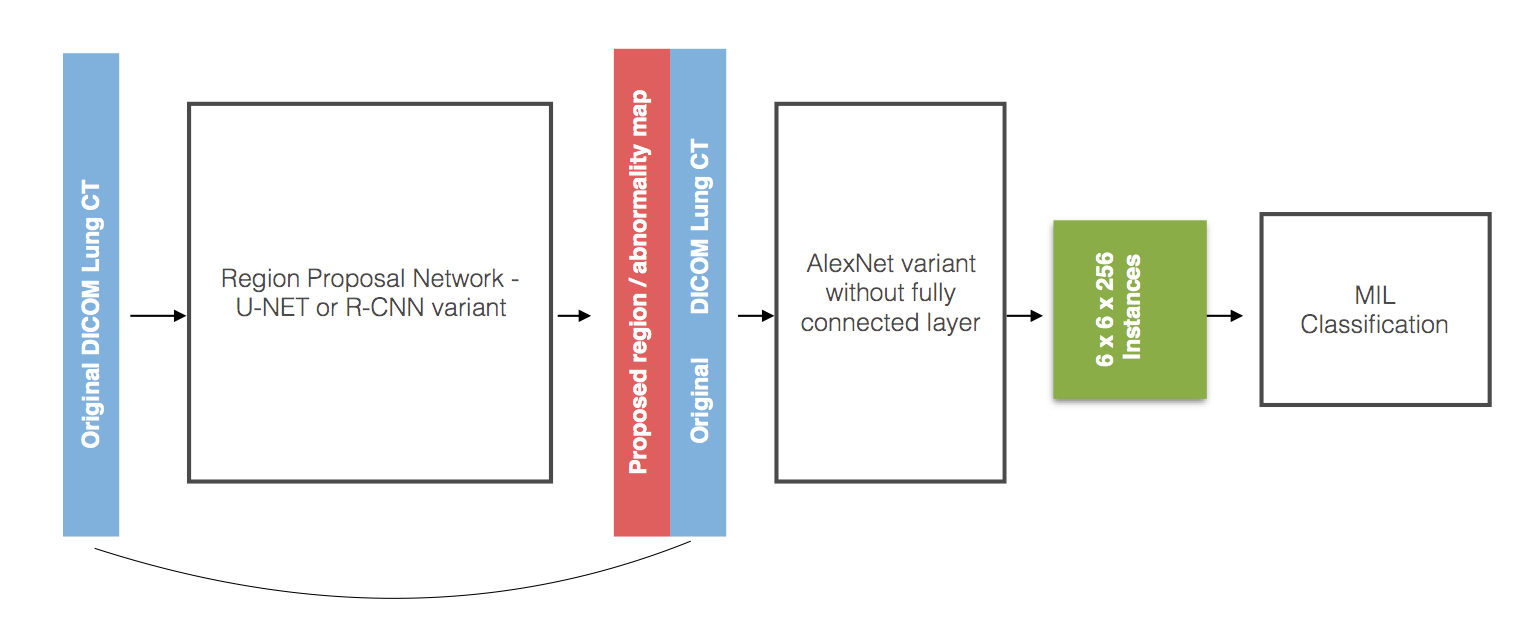
\includegraphics[width=\columnwidth]{img/architecture.png}


We plan to leverage state of the art region proposal and biomedical segmentation
to indicate nodule presence and implicitly weight instances consumed by a 
downstream Multi-Instance Network (MIN) classifier.

In our pipeline, a region proposal network is trained on the LUNA dataset to propose
nodule annotations and abnormal regions in CT slices. This region proposal 
is then used to annotate nodules in Kaggle dataset. Then a MIN classifier based 
on the work on mammogram  classification by Lou et. al \cite{DBLP:journals/corr/ZhuLVX16},
will be trained on the annotated Kaggle dataset.

\subsection{Training}
We will train the upstream and downstream networks seperately. Once the upstream,
region proposal/segmentation network is trained, we will then replace the last layers
of the upstream network with convolutional layers to learn the features that best
associate region proposals with malignancy.

\subsection{Choosing the Region Proposal Network}
We have several region proposal networks we want to investigate.
We will tune one segmentation/region proposal network for our final pipeline. 
the region proposal networks that we suspect will yield promising results can 
be classified int two categories.

First, there exists segmentation networks based of U-Net, a seminal CNN for biomedical
segmentation developed by Brox et. al \cite{U-net_2015}. The most easily accessible
U-Net based pipeline for supervised biomedical image segmentation is 
a pre-trained network, available on Caffe Model Zoo, for CT Liver Lesion 
segmentation \cite{DBLP:journals/corr/ChristEETBBRAHD16}.

Second, there exists other highly successful, and fast, region proposal and 
segmentation networks developed for non-biomedical domains. We
will test the fully convolutional neural network developed by Darrell et. al at
Berkeley \cite{long_shelhamer_fcn} (Jay and Jason will be investigating this network as a paper 
presentation). We will also test and try to adapt Faster R-CNN developed by He 
et. al \cite{fast_rcnn_2015, faster_rcnn_2015} for nodule detection.

Recent U-Net based segmentation leverage depth information whilst non-biomedical
region proposal and segmentation networks do not use depth information. If time permits or
if we deem necessary, we will attempt to adapt successful 2D methods to work in 3D. 


%%%% This paragraph is better in this section, but (jason) can't quite make it flow/work

% In our pipeline we first deal with module detection. For this step there are a 
% number of related papers in particular we will look at U-net for a biologically 
% adapted segmentation algorithm \cite{U-net_2015}. U-net seems to be a fairly 
% simple 2d CNN model that makes most of its gains in data augmentation it is 
% likely that we will be able to use these biologically sound data augmentation 
% techniques with a slightly more sophisticated model that is based on 3d 
% assumptions, something like the 3d CNN trained on weakly labeled data last 
% year at Arizona State University \cite{LungNoduleDetectionWeaklyLabeled_2016}. 
% Region proposal networks such as fast and faster r-cnn may also apply here 
% \cite{fast_rcnn_2015, faster_rcnn_2015}. We will also investigate other 3d 
% segmentation techniques such as the combination of fully convolutional networks 
% and recurrent neural network by researchers at Notre Dame last year could apply 
% here \cite{fcnn_and_rnn_3d_bio_2016}. Some other interesting papers 
% \cite{CNN_Segmentation_Medical_Imaging_2017, Lai_2015}

\subsection{The Multi-Instance Network}

We will adapt Multi-Instance Network (MIN) developed for mammogram classification developed by
Lou et. al \cite{Maron:1998:FML:302528.302753} to lung cancer detection. 
Their implementation feeds the 6 by 6 by 256 output of the last
convolutional layer of AlexNet as instances to three Multi-Instance (MI) loss functions 
that are then aggregated into a final loss.

We will use the same architecture and first use 2D instances to look for 
lung cancer. If time permits, we will adapt the MIN to instead use 3D, voxel
based convolutions as the output instances for MI loss functions. 

We particularly like this AlexNet variant because, amongst the team, we own and 
have access to two NVidia GTX 970 4GB GPUs.

\subsection{Data Augmentation}

One major challenge we will face will be the fact that we have a very small 
collection of data. We plan to heavily augment our data. Inspired by the MIN
for mammogram classification, we plan to apply a new random set of augmentation
to each epoch of training data.

\section{Datasets}
The number of lung CT scans available to us is very low. The total number of examples
available are many orders of magn{}itudes smaller than the size of datasets for modern,
state of the art classification challenges such as ImageNet or MSCOCO.

Listed below are the datasets we will leverage to train our classification/nodule
extraction model.

\begin{center}
\begin{tabular}{lll}
  \toprule
  Dataset & \# CT scans & Label Type\\
  \midrule
  Kaggle&1398&Cancer/No-cancer\\
  LIDC-IDRI&1018&Nodule annotation\\
  SPIE&80&Nodule annotation\\
  NLST&?&?\\
\end{tabular}
\end{center}

In the dataset above, each CT scan is a stack of 
approximately 200 2D slices.

The Kaggle dataset will be obtained from the Kaggle Data Science Bowl 2017
competition. The dataset consists of over 1000 CT scans in DICOM format labeled
by a cancer/no-cancer binary. We will use this data train our downstream
 MIN classifier.

The Lung Image Database Consortium (LIDC-IDRI) dataset is the dataset used in 
the 2016 LUNA challenge.The dataset consists of over 1000 CT scans where
each nodule location and radius is annotated for each 2D slice. The dataset was
annotated by 4 radiologists and nodules are annotated with varying levels of 
agreement. We will use this dataset to train our upstream region/nodule 
proposal network.

The SPIE dataset is a minuscule but have a few important examples where nodules
are both annotated and labeled benign or malignant. This dataset may help us 
validate and visualize the convolutions happening in both the upstream
region/nodule proposal and downstream MIN classifier.

We suspect that the National Lung Screening Trial (NLST) dataset will contain 
about another 1000 CT scans that will either be labeled with the 
cancer/no-cancer or nodule annotations. We have applied for and are
currently waiting for access to the NLST data.

\section{Evaluating our results}

\subsection{Our goals}
We have two primary goals in this investigation. First we want to know if region
proposal and implicit instance weighting aid multiple instance learning. Second,
we want to investigate how leveraging depth information from our data helps
with inference with biomedical imaging.

\subsection{How will we know what is going on?}
% \temp{
%   - visualize 2D convolutions in both upstream and downstream nets \\
%   - visualize 3D convs if we get to it in the downstream MIL net \\
%   - Use SPIE data to see how malignant vs benign tumors are `seen' by our network\\
% }

The SPIE dataset will give us insight as to how our network sees both benign
and malignant nodules or tissues. We hope to visualize both 3D and 2D convolutions
in both upstream and downstream networks.

\subsection{Quantifying our results}
% \temp{
%   - COMPARE FASTER R-CNN with U-NET and other segmentation methods\\
%   - Figure out how the upstream region output effects downstream classifier\\
%   - Compare direct MIL classification with region enhanced MIL classification\\
% }

We think that one of the most important contribution this investigation will make
is how we can perform biomedical inference with small datasets that are not
labeled homogeneously.
Our network architecture allows us to plug and play, and even remove, upstream
region proposal networks. 

We can test different region proposal techniques and quantify how upstream
region proposals affect weakly labeled Multi-Instance Networks. We can then
also quantify what effects these upstream techniques have on false positive and
false negative classifications.

One aspect to focus on specifically is the weight balance on the MI network
between the region proposal data and the CT scan data. The proportion of
weight allocated to each layer after training leads to some insight about how
much the network uses the region proposal information in the final prediction process.

\section{Results}

\subsection{Evaluation of segmention methods}

\newcommand{\tbox}[1]
{\noindent\fbox{\parbox[c][5cm][c]{\columnwidth}{\begin{center} #1
\end{center}
}
\vspace{0.5cm}
}}

\red{Graphs to be prepared by April 21st}

\tbox{Loss vs Epoch for multiple segmenation networks with LUNA data}

\tbox{Table of segmentation metrics, with IOU and pixel accuracy}

\subsection{Visualizations for segmentation}

\tbox{Ground truth vs output visualizations for good cases}

\tbox{Ground truth vs output visualizations for bad cases}

\section{Overall evaluation}

Here, we evaluate the effect of upstream ROI proposals. We graph loss over
epoch for each of our classifiers with different upstream networks. We also
compare these networks with a vanilla classifier without upstream ROI proposals.

We will produce graphs below with Kaggle validation data.

\tbox{Loss vs Epoch for different classifiers}
\tbox{Precision vs Recall curves for different classifiers}
\tbox{ROC curves}
\tbox{Table of AUC and accuracy}

\section{About us}
\subsection{Jay DeStories}
Jay is working with Prof. Guyer on graph inference for social
marketplaces. His background is primarily in systems and web engineering.

\subsection{Jason Fan}
The resident math major. Jason is currently working with Prof. Hescott on Graph
related kernalized learning. Unfortunately, Jason the only team member 
who has failed to earn his master's in his fourth year of his undergraduate career.
Jason has lead the writing process so far.

\subsection{Alex Tong}
Alex works with Prof. Hassoun on metabolomics. He is most interested in 
investigating the effects of the region proposal prior on the performance of
the disease prediction network, in relation to models of visual attention \cite{NIPS2014_5542}. 

\subsection{The Team}
In the team, Jay and Jason have already partnered up to investigate a
fully convolutional image segmentation technique and will take the lead on
adapting region proposal methods to nodule detection. They also own the
two GPUs :).

Alex will take the lead in the downstream MIN and investigate other MI loss 
functions that can enhance cancer detection as well as the effect of region 
proposal on overall MI network performance.

\bibliographystyle{unsrt}%Used BibTeX style is unsrt
\bibliography{proposal}
\end{document}
